\section{Orientation histogram detector}

\subsection{Introduction}

    I first built a detector to detect the robot position and orientation. 
    To do so, I used a histogram detector to detect three dots and calculate
    the angle of the height of the triangle. In order to work properly, two 
    points must be clearly closer to form a triangle that is near to be 
    isosceles. (drawing)

\subsection{Detection of the object and his orientation}

    \marginpar{
        \captionof{figure}{Calculation of the orientation}
        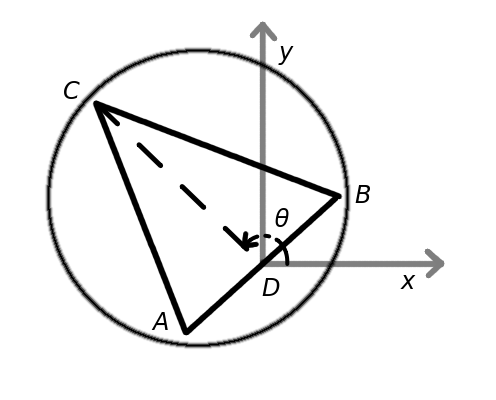
\includegraphics[width=5cm]{./img/orientation.png}
        The orientation $\theta$ is the angle between the
        line $\overline{CD}$ and the $x$ axis. It ranges
        counterclockwise from 0 to 2$\pi$.
    }

    \marginpar{
        \captionof{figure}{Calculation of the orientation}
        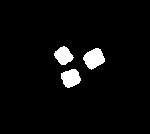
\includegraphics[width=4.5cm]{./img/OrientationDetector_detect.png}
        The orientation $\theta$ is the angle between the
        line $\overline{CD}$ and the $x$ axis. It ranges
        counterclockwise from 0 to 2$\pi$.
    }

    \marginpar{
        \captionof{figure}{Calculation of the orientation}
        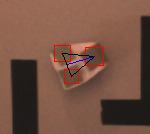
\includegraphics[width=4.5cm]{./img/OrientationDetector_image.png}
        The orientation $\theta$ is the angle between the
        line $\overline{CD}$ and the $x$ axis. It ranges
        counterclockwise from 0 to 2$\pi$.
    }
 
    The detector first detects blobs with the help of the histogram 
    detector. When this is done, it iterate through the blobs and selects 
    the three biggest ones.  It then selects the two closer points and 
    calculates the line from D to C to get the angle theta, which is the 
    orientation of the object.
   \\
    \\
    The position of the object is the mean position of the three points.

\subsection{Improvements}

    The detector is weak to noise. If one of the dots is not correctly 
    detected and get smaller than some noisy blobs, the noisy blob is 
    detected as one of the dots and the calculated position is not 
    good.

    We could keep the three points in memory and take the closest points 
    at the next detection. It could still be unstable if the movement is 
    fast and noise is closer than the next position. The best option may 
    be to weight the distances with the size of the blobs. 
    \\
    \\
    The detector was to unstable because of small changes in ambient light.
    Also, we needed to remove the Khepera from under the camera every time 
    we restarted the detector, because the histogram should not contain 
    colors of the Khepera. So I decided to build a new detector that would 
    detect specific colors. This way, the detector would be more reliable 
    or could me more easily reconfigured during ambient light changes. 
    Also, we could also leave the Khepera under the camera all the time. 
    \\
    \\
    The Orientation histogram detector is not included in Tapir because 
    the Orientation color detector works better on every aspects, so the 
    one is useless.

\subsection{How to use}
    \begin{enumerate}
        \item Find a color that is well detected with the detector in the desired environment.
        \item Put 3 dots of the found color on the object you want to detect (square of colored paper seems to fare better than colored dots with pencils on white paper)
        \item Get the object out of the vision
        \item Start the detector and wait a few second until it stops adding frames to the histogram
        \item Add the object to the environment. 
    \end{enumerate}

    \marginpar{
        \captionof{figure}{Calculation of the orientation}
        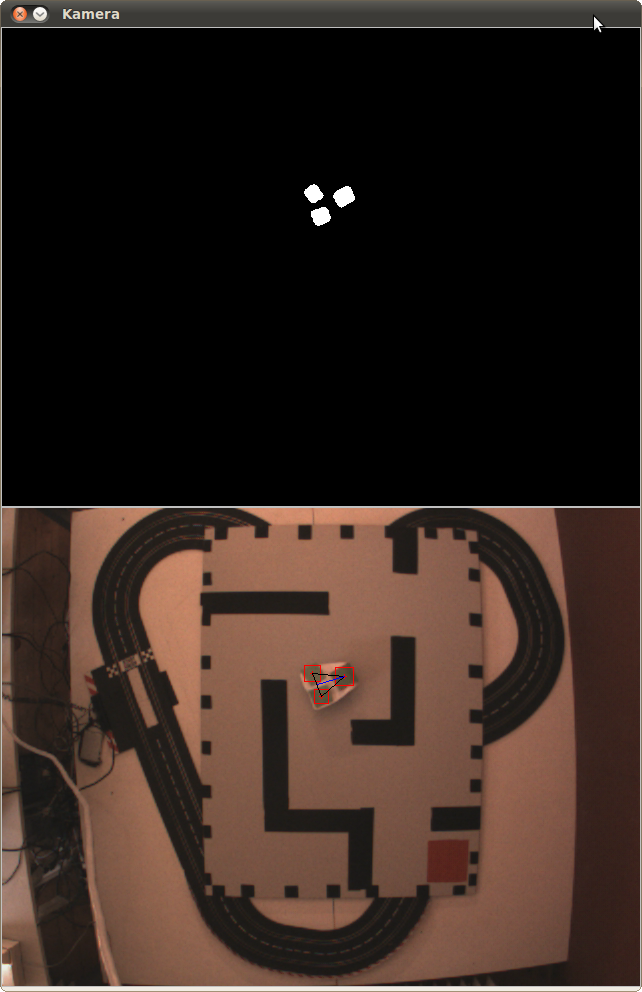
\includegraphics[width=4.5cm]{./img/OrientationDetector_full.png}
        The orientation $\theta$ is the angle between the
        line $\overline{CD}$ and the $x$ axis. It ranges
        counterclockwise from 0 to 2$\pi$.
    }
 

\subsubsection{Parameters for configuration file}
    \begin{description} \itemindent=-15pt
        \item[examples\_init] \hfill \\ number of frames added to the histogram at the beginning
        \item[examples\_renew] \hfill \\ number of frames added to the histogram when pressing ‘+’
        \item[box] \hfill \\ draw box around all blobs in the image
        \item[area] \hfill \\ (min,max) define minimum and maximum size to detect objects (objects smaller than min or bigger than max are not detected)
        \item[filename] \hfill \\ filename where to save histogram (optional)
        \item[autoload] \hfill \\ load the histogram saved in ‘filename’ at the beginning
    \end{description}

\subsubsection{Keys}
    \begin{description} \itemindent=-15pt
        \item['+'] \hfill \\ add 'examples\_renew' frames to the histogram
        \item[' ' (space)] \hfill \\ add frames to the histogram until ' ' (space) his pressed again.
        \item['s'] \hfill \\ save the histogram in 'filename'
        \item['l'] \hfill \\ load the 'filename' histogram
    \end{description}

